\chapter{Mesh generation and CFD solver}
\label{solver}

In a recent decade, the capability of computational analysis and optimization has made considerable improvement, which made many researchers rethink solutions to real-world problems. One such problem addressed here is the optimization of wing surface geometry. There requires several software packages and link them using some tools to address these problems. In the entire process of wing shape optimization, the bottleneck is found to be a CFD solution. More importance needs to be given to minimize the time taken by the solver. The SU2 solver is chosen based on its ease of availability and other constraint involved. The solver is initially tested on sample wing shape (NACA 0012 wing) for its reliability, and results seem positive. Also, the SU2 solver is open-source. Hence, more flexibility will be available to tweak the code. In this chapter, the emphasis is given to implement the SU2 solver and Pointwise (meshing software).

\section{Mesh generation}
The work presented in this thesis involves the use of proprietary software called Pointwise for mesh generation. This software provides the flexibility of using well-known scripting languages like python and tcl (tool command line) for mesh generation, which is the crucial feature that makes it possible for 3-D shape optimization. Also, it exports the mesh file in su2 format. More information about the mesh size will be mentioned in chapter \ref{results}.

In this work, after obtaining the perturbed wing surface coordinates in Plot3D format, it is subjected to volume mesh generation. A glyph script is constructed for volume mesh generation, and it can be accessed using the link mentioned here, \href{https://github.com/neelu065/M-Tech_project_code/blob/master/Project_code_fNRAND1/optimizer_input/pointwise_mesh_template.glf}{\underline{\textit{pointwise glyph script}}}. 

The script initially imports the perturbed wing coordinates (*.x3d), which was generated using the principal components of the sampled wings. It is known that winglets will reduce the induced drag without actually increasing the aspect ratio of the wing. Thereby, the cumulative lift is increased. An attempt is made to club the winglet formation before the wing is imported into meshing software. However, this method faced difficulty obtaining the winglet, as winglets need to be adaptive with the wingtip section. There cannot be a universal winglet that fits all generated perturbed wings inside the generation. Altogether, the winglet creation needs to be automated based on the shape of the wingtip section of a given wing.

After importing the perturbed wing to pointwise using glyph script, the next step is to make the script identify the wingtip section. There are several ways, namely, identifying the extreme points of a connector which connects the wing root section and tip section or identify by connector names. 

\subsection{Winglet creation}
This work follows identifying the wingtip section curve by connector name (in this work, it was con-2). The connector (con-2) is split at its leading edge point, which is identified by finding the minimum coordinate value in the curve (con-2) in the chord direction. With this, the wingtip curve is split into two halves (con-2-split-1,con-2-split-2) at the identified minimal point. Figure \ref{connector_split} represents the same. 

\begin{figure}[!htbp]
    \centering
    \framebox{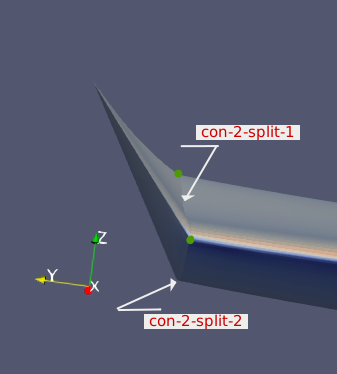
\includegraphics[scale = 0.4]{figures/winglet_1-check.png}}
    \caption{Wingtip connector split into two halves.}
    \label{connector_split}
\end{figure}

Then, calculate the dimension (number of mesh points) of either of the split curves. To construct the winglet, initially, the winglet curve is to be constructed. A minimum of three points is required to define a curve. Among them, two points are the end of the wingtip curve (con-2), whereas the third point (also called a shoulder point) coordinate is evaluated as follows,
\begin{itemize}
\item Along chord direction (x-coordinate): The weighted average of the x-coordinates of extreme points in the wingtip section curve. However, weight is user-defined. A weight of 25\% and 75\% are provided to extreme x-coordinates of the curve (con-2-split-1).
\item  Along span direction (y-coordinate): The y-coordinate of the shoulder point will be 2\% of the given wingspan, that is, $1.02s$, where $s$ is span length.
\item Along thickness direction (z-coordinate): The z-coordinate of the shoulder point is crucial. A wrong calculation of this coordinate will lead to an unrealistic winglet. In this work, the slope of the curve (con-3) connecting the wingtip and wing root section is evaluated. Further, the z-coordinate is obtained by the method of extrapolation, using the slope obtained and the 2\% of span length$(s)$.
\end{itemize}

\begin{figure}[!htbp]
\parbox{0.5\linewidth}{
    \centering
    \framebox{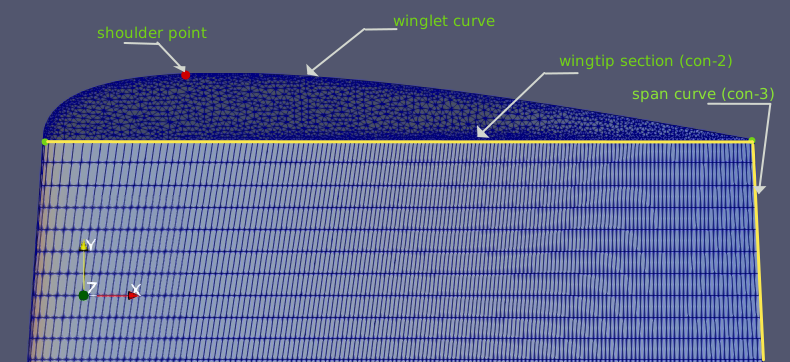
\includegraphics[scale = 0.3]{figures/winglet_frontview.png}}
    \caption{Winglet frontview.}
    \label{winglet_frontview}
}
\parbox{0.5\linewidth}{
   \centering
    \framebox{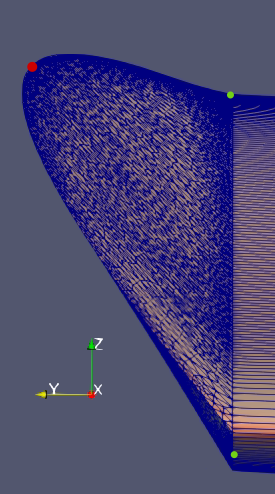
\includegraphics[scale = 0.4]{figures/winglet-sideview.png}}
    \caption{Winglet sideview.}
    \label{winglet_sideview}
}
\end{figure}
Figure \ref{winglet_frontview} depict the same. The red color dot represents the shoulder point. A curve is generated using three points is named as a winglet curve. The dimension of the winglet curve is set equal to either of con-2-split-1 or con-2-split-2. An unstructured mesh is generated between the winglet curve and the wingtip section curve (con-2). The outcome is shown in figure \ref{winglet_sideview}. Green colored dots represent the extreme mesh points along the wingtip section.  

\subsection{Volume mesh generation}
Once the winglet generation is completed, the surface mesh is subject to volume mesh generation. In this work, the T-Rex method is implemented to generate the volume mesh. This method was introduced in Gridgen in the year 2007 and has seen several improvements continuously. T-Rex generates hybrid meshes that resolve boundary layers, wakes, and other phenomena in viscous flows by extruding layers of high-quality, high aspect ratio tetrahedra that can be post-processed into stacks of prisms. The algorithm includes tools for optimizing cell quality and avoiding collisions of adjacent layers of cells. More on this can be found in the link mentioned here, \href{https://www.pointwise.com/theconnector/2011-July/T-Rex-Hybrid-Meshing-Pointwise.html}{\underline{\textit{T-Rex}}}.

\begin{figure}[!htbp]
    \centering
    \framebox{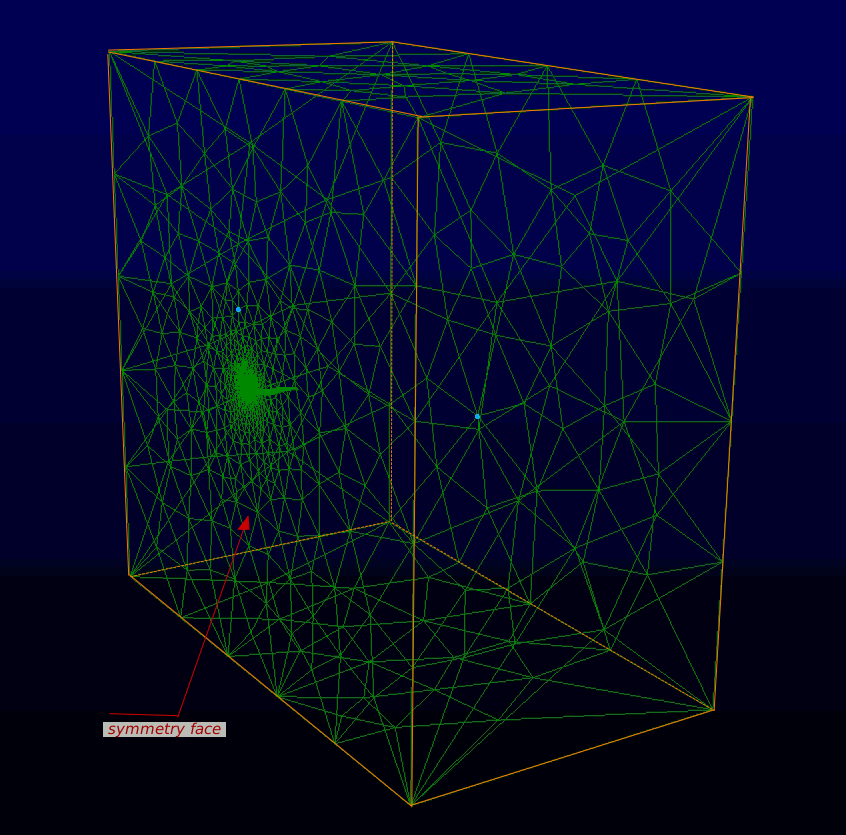
\includegraphics[scale = 0.3]{figures/volume_mesh.png}}
    \caption{T-Rex mesh}
    \label{T-Rex}
\end{figure}
The T-Rex method involves setting the boundaries around the wing surface. The literature shows that a scale factor of 15 units (1 unit = 1 chord length) would be sufficient to cover all the wake region, and the far-field boundary surface would look similar to the one shown in figure \ref{farfield}. A distance of 15 units is available on both the leading edge side, trailing edge side, and the span direction. A  growth factor of 1.2 is set, and the T-Rex mesh generation is initialized. The outcome of the T-Rex mesh is shown in figure \ref{T-Rex}.

\begin{figure}[!htbp]
    \centering
    \framebox{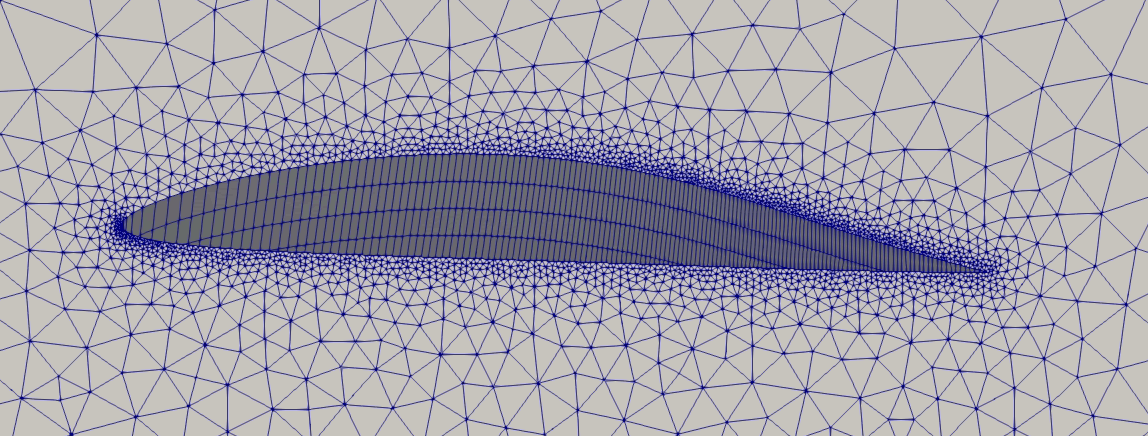
\includegraphics[scale = 0.35]{figures/airfoil_mesh.png}}
    \caption{Mesh around one of perturbed wing sectioned at symmetry plane.}
    \label{airfoil_mesh}
\end{figure}

The number of mesh points in the T-Rex depends on the wing surface mesh points, the growth rate of the mesh, and the full layers selected. This work contains no full layers and has a single block mesh. In the previous work, researchers attempted to implemented multi-block mesh to these problems. However, while addressing these problems, setting up the multi-block mesh seems intricate. Moreover, building the script which creates the multi-block mesh to all perturbed wings is a difficult task. A mesh generated over the airfoil section at symmetry is shown in figure \ref{airfoil_mesh}.

\begin{figure}[!htbp]
    \centering
    \framebox{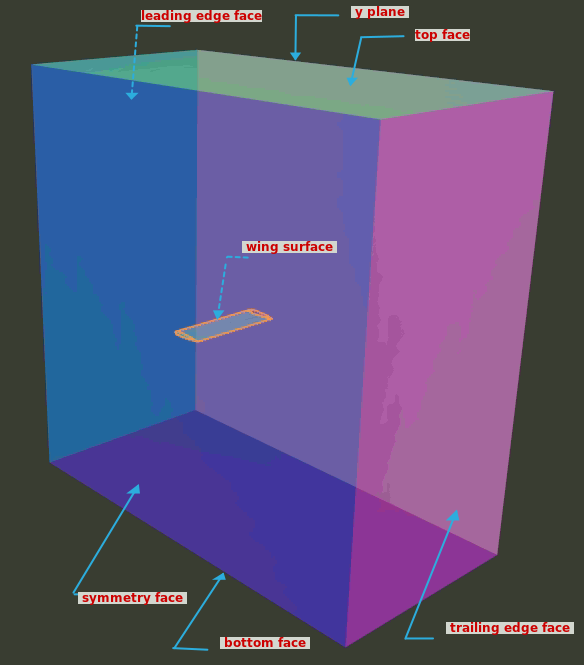
\includegraphics[scale = 0.4]{figures/wing_body.png}}
    \caption{Far field boundaries.}
    \label{farfield}
\end{figure}

Now, each of these far-field faces is assigned a specific name that will assist the solver in interpreting and assigning the boundary condition values. Table \ref{boundary_surface_values} refer the same.

\begin{table}[!htbp]
    \centering
    \begin{tabular}{|c|c|}\hline
    \textbf{General values}     &  \textbf{Boundary surface value}\\\hline
    Leading edge face     &  X{NORMAL}\textunderscore{FACES}\\
    Trailing edge face    &  X{NORMAL}\textunderscore{FACES} \\
    Top face              &  Z{NORMAL}\textunderscore{FACES} \\
    Bottom face           &  Z{NORMAL}\textunderscore{FACES} \\
    Y-plane               &  Y{NORMAL}\textunderscore{FACE} \\
    Symmetry face  & SYMMETRY \\
    Wing surface (including winglet) & WALL \\\hline
    \end{tabular}
    \caption{Boundary surface values}
    \label{boundary_surface_values}
\end{table}

After setting the boundary surface name, the volume mesh is exported in the su2 format (*.su2). However, the numerical values for boundary surfaces will be assigned in the solver configuration file, which is explained in the upcoming section. 

\section{CFD solver}
After the check over a few CFD packages like CFD++, ANSYS, and SU2, it is decided to use the SU2 solver for the CFD simulation. The reason for the choice is that the SU2 solver is an open-source project and can be installed in clusters without admin permissions. Other CFD packages require licenses, and limited licenses may cause license error when other users are using it.

The SU2 suite is an open-source collection of C++ based software tools for performing Partial Differential Equation (PDE) analysis and solving PDE-constrained optimization problems. The toolset is designed with Computational Fluid Dynamics (CFD) and aerodynamic shape optimization in mind. More information about solver can be found in the link mentioned here, \href{https://su2code.github.io/docs_v7/home/}{\underline{\textit{SU2 solver}}}.

The sample script of solver configuration is mentioned here,
\href{https://github.com/neelu065/M-Tech_project_code/blob/master/Project_code_fNRAND1/optimizer_input/template.cfg}{\underline{\textit{solver configuration file}}}. The CFD solver setup is straight forward. The variable called MACH\textunderscore{NUMBER} is used to set up the free stream Mach number. A similar approach is carried to other variables too. Since the SU2 solver provides more features for ASO, one such feature optimizes the lift coefficient based on the change in the angle of attack. In this work, the problem demands a lift constraint of 0.2625, and the value can be optimized with this help of solver alone. 

The template contains the variable suffix called MARKERS, which refers to boundary condition value, as mentioned in table \ref{boundary_surface_values}. The solver output contains a vast amount of aerodynamic data. Extracting the required data from the output file makes it possible to optimize the wing surface and assist in moving to the next generation. The solver also offers the output in both data format (*.csv) and the visualization format (Paraview, Tecplot). It even has the feature of restarting the solution. However, this work does not require the use of restarting the solution.

\section{Boundary conditions}
Equation \ref{euler_equation} represents the 3-D inviscid fluid flow governed by the Euler equation.
\begin{equation}
\frac{\partial \mathrm{Q}}{\partial t}+\frac{\partial \mathrm{E}}{\partial x}+\frac{\partial \mathrm{F}}{\partial y}+\frac{\partial \mathrm{G}}{\partial z}=0
\label{euler_equation}
\end{equation}
where,\\
\textbf{Q} is a vector of conservative flow variables,\textbf{ E}, \textbf{F}, and\textbf{ G} are convective flux vectors.

Table \ref{boundary_surface_values} represents the boundary surface values shown in figure \ref{farfield}. Free stream flow direction across the XNORMAL\textunderscore{FACES}, and there exist no crossflow across ZNORMAL\textunderscore{FACES} and YNORMAL\textunderscore{FACE}. Both SYMMETRY and WALL surfaces are assigned to Euler wall conditions (no-slip condition). The XNORMAL\textunderscore{FACES}, YNORMAL\textunderscore{FACE}, and ZNORMAL\textunderscore{FACES} are farfield boundaries. The CFD solver is set at a Mach number of 0.4, free stream pressure of 1 atmosphere, and at free stream temperature of 288K. The initial angle of attack is set to be 3$^0$. However, as mentioned, the lift coefficient constraint is achieved by perturbing the angle of attack. From trial and error, it is noted that the CFD iteration of 3000 would be sufficient to converge the solution to the residual order of $-8$. More on this is mentioned in chapter \ref{results}.

\section{Job submission}
Optimization is a computationally expensive process. A proper computation facility is required to carry out such a process. In this work, during the testing phase of optimization codes, the work is carried out in the workstation, with ten cores (20 CPU). However, this is noted that this will not be sufficient to submit the entire optimization code. Then the work is shifted to the HPC cluster, where sufficient resource was available.

Every CFD simulation is a time consuming expensive computational process. As a result, the handling of each simulation (as called a job) is necessary.  A scheduling package called SLURM (Simple Linux Utility Resource Management) is used to address this. More on this can be found in the link, \href{https://slurm.schedmd.com/overview.html}{\textit{\underline{SLURM}}}.

A sample template used for job submission is shown here, \href{https://github.com/neelu065/M-Tech_project_code/blob/master/Project_code_fNRAND1/optimizer_input/submit_jobs.sh}{\underline{\textit{slurm script}}}. In the initial days of the project, it was planned to submit each CFD simulation as an individual job to the compute node using the SLURM script. However, the restrictions did not allow this to take place. With further modifications to the python optimization code, each generation is submitted as an individual job. Every job demands 20 CPU (population size is 20), and each CPU will carry out the CFD simulation on each perturbed wing in a given generation. This process repeats for the entire set of generation cycles. 

\section{Conclusion}

In this chapter, detailed information about the mesh generation (particularly volume mesh) is explained. The creation of a winglet was a tedious job and involved a considerable amount of time. Setting up the boundary values are straight forward. The mesh quality, inlet boundary conditions and free stream conditions are not explained here. They will be addressed in chapter \ref{results}. The selection of CFD solver and the reasons for its choice is mentioned. Finally, the way each simulation is fired into compute nodes is mentioned. For all the work mentioned above, proper scripting is involved. The template scripts referring to each of them are linked in the respective sections.   